% ============================================================
% OUTLINE -- Appendix     unlimited pages; supplementary only.
% Nothing here is required to follow the 4-page main text.
% Sections become A, B, C, ... under \appendix (set in
% acl_latex.tex).
% ============================================================

\section{Proof of the Telescoping Identity}
\label{app:proof}
% - Full statement and proof that sum_t r_t = recall@K(\hat{L}_R) -
%   recall@K(\hat{L}_0) under equal add/drop weights, and that
%   potential-based shaping \citep{ng1999policy} leaves the
%   optimal policy invariant -- so the dense objective and the
%   recall@K optimum coincide.
% - Regret view: Case 1 (a gold-for-gold swap) has regret 0;
%   Case 2 (a non-gold kept over a gold) has regret 1.

\section{Code Graph Construction}
\label{app:graph}

The scaffolding's neighborhood expansion
(Section~\ref{sec:scaffold}, Step~B) walks a per-repository
code graph $\mathcal{G}{=}(V,E)$. We follow the four-edge
schema of \citet{chen2025locagent} as implemented in
\citet{chaudhari2025spider}, summarised here for completeness.

For each repository the graph is built from the source files
written in the repository's primary language; files in
secondary languages are ignored. Nodes represent code entities
at four granularities (directory, file, class, and function),
and edges encode four structural relations: a \textit{contains}
edge linking each container to the code units it declares, an
\textit{invokes} edge between a function and each function it
calls, an \textit{imports} edge between a file and each module
it imports, and an \textit{inherits} edge between a class and
each parent class it extends. Every non-directory node stores
its source text alongside its identifier, so the model can see
code when a node is shown.

We extract Python source files with the standard \texttt{ast}
module and Java, JavaScript, and TypeScript files with
Tree-sitter\footnote{\url{https://github.com/tree-sitter}}. The
traversal of the repository's directory tree adds directory
nodes for navigation, skips files that contain no class or
function definition, and emits one node per declared entity
together with its containment, call, import, and inheritance
edges. Multi-file class definitions and the more flexible
declaration patterns of the non-Python languages are handled
with language-specific Tree-sitter queries; we refer to
\citet{chaudhari2025spider} for the full list of cases. Graphs
are constructed on demand at the start of a localization run
and reused across the rounds.

For the experiments in Section~\ref{sec:experiments}, we use
the graphs released with \citet{chaudhari2025spider} for
SWE-PolyBench and SWE-Bench Verified, and construct graphs from
scratch for the SWE-Bench Lite dev split with the same
pipeline.

\section{Scorer Training Details}
\label{app:details}

This appendix complements Section~\ref{sec:training} with the
hyperparameters and procedural details that we omit from the main
body.

\paragraph{Group construction.}
For each issue, every ground-truth function that falls inside the
retriever's top-$N$ pool is included as a positive; the group is
then completed to size $M$ with non-relevant candidates. Negatives
are drawn with a stratified strategy: a fixed fraction is taken as
top-ranked hard negatives, and the remaining slots are filled by
partitioning the rest of the pool into equal-width rank bins and
sampling one negative per bin. Each group therefore exposes the
model to shallow, mid- and deep-pool negatives, which empirically
prevents the calibration drift on deep-pool non-relevant candidates
we observed under top-only hard-negative sampling. Negatives are
re-sampled at the start of every epoch, so depth coverage widens
monotonically across training.

\paragraph{Optimization.}
The adapter is trained in bfloat16 with FlashAttention-2 and
activation checkpointing on the backbone. AdamW is used with the
schedule of Table~\ref{tab:hparams}; gradients are accumulated over
$8$ groups before each optimizer step and clipped to unit norm. All
$M$ candidates of a group are forwarded under autograd in a single
optimizer iteration so that the listwise term in~\eqref{eq:cov}
backpropagates jointly across the group.

\paragraph{Distributed training.}
Training is data-parallel across GPUs via Hugging Face Accelerate.
At the start of each epoch the shuffled issue list is sharded into
disjoint contiguous slices --- one per rank --- and each rank
builds its own training groups independently. Because issues whose
ground-truth functions fall outside the retriever pool are dropped,
the per-rank post-filter group counts are reduced with a
min-collective to keep DDP collectives aligned. LoRA gradients are
small relative to the backbone, so all-reducing them on every
backward is inexpensive and we do not shard the model.

\paragraph{Evaluation during training.}
After each epoch the current adapter is evaluated on a fixed
held-out subset of validation issues using the same windowed
top-$K$ procedure as inference: candidates are scored in sliding
windows over the top-$N$ pool, the global top-$K$ by score is
selected, and function- and file-level $\text{recall}@K$ are
reported. Best-epoch selection on this validation metric determines
the adapter shipped for the test-time evaluation in
Section~\ref{sec:experiments}.

\paragraph{Prompt format.}
The training-time prompt format matches the inference scorer's
format exactly, including the assistant-turn template and the
position at which the \textsc{yes}/\textsc{no} logits are read.
Mismatches between train- and test-time prompts silently shift the
score distribution and are the most common source of regression
when porting the adapter to a new backbone.

\begin{table}[h]
\centering
\small
\caption{Scorer fine-tuning hyperparameters. The same
configuration is used for the BCE-only ($\lambda{=}0$) ablation
and the main BCE+coverage ($\lambda{=}0.2$) runs.}
\label{tab:hparams}
\setlength{\tabcolsep}{4pt}
\renewcommand{\arraystretch}{1.05}
\begin{tabular}{ll}
\toprule
\textbf{Component} & \textbf{Value} \\
\midrule
Backbone               & Qwen2.5-Coder-3B-Instruct \\
                       & \citep{hui2024qwen25codertechnicalreport} \\
Precision              & bfloat16, FlashAttention-2 \\
Adapter                & LoRA, $r{=}4$, $\alpha{=}32$, dropout $0.05$ \\
LoRA targets           & $\{q,k,v,o\}_{\text{proj}}$, \\
                       & $\{\text{gate},\text{up},\text{down}\}_{\text{proj}}$ \\
Score readout          & $s = \ell(\text{yes}) - \ell(\text{no})$ \\
                       & at final prompt position \\
Group size $M$         & $20$ candidates per issue \\
Issue / code trunc.    & $3072$ / $1024$ tokens \\
Negative sampling      & $40\%$ top hard negatives; \\
                       & remainder one-per-bin across pool; \\
                       & re-sampled each epoch \\
BCE class weights      & $w_{+}{=}w_{-}{=}1$ \\
Coverage weight        & $\lambda{=}0.2$ (main); $\lambda{=}0$ (ablation) \\
Optimizer              & AdamW \\
Learning rate          & $1{\times}10^{-4}$, cosine, $3\%$ warm-up \\
Grad. accumulation     & $8$ groups per step \\
Grad. clipping         & max norm $1.0$ \\
Epochs                 & $5$ \\
Retriever pool $N$     & $500$ \\
Train / val split      & $95\%/5\%$ of issues, fixed seed \\
\bottomrule
\end{tabular}
\end{table}

\section{Additional Results}
\label{app:results}

The figures below complement the function-level scorer
evaluation reported in
Section~\ref{sec:main-results} (Figure~\ref{fig:scorer-func-recall}).
Both use the same windowed protocol on SWE-PolyBench: the
first-stage retriever returns the top $\text{PS}{=}100$
candidates, the scorer ranks a window of $K{=}20$, and the
top-$L{=}5$ by score are selected.

\begin{figure*}[t]
\centering
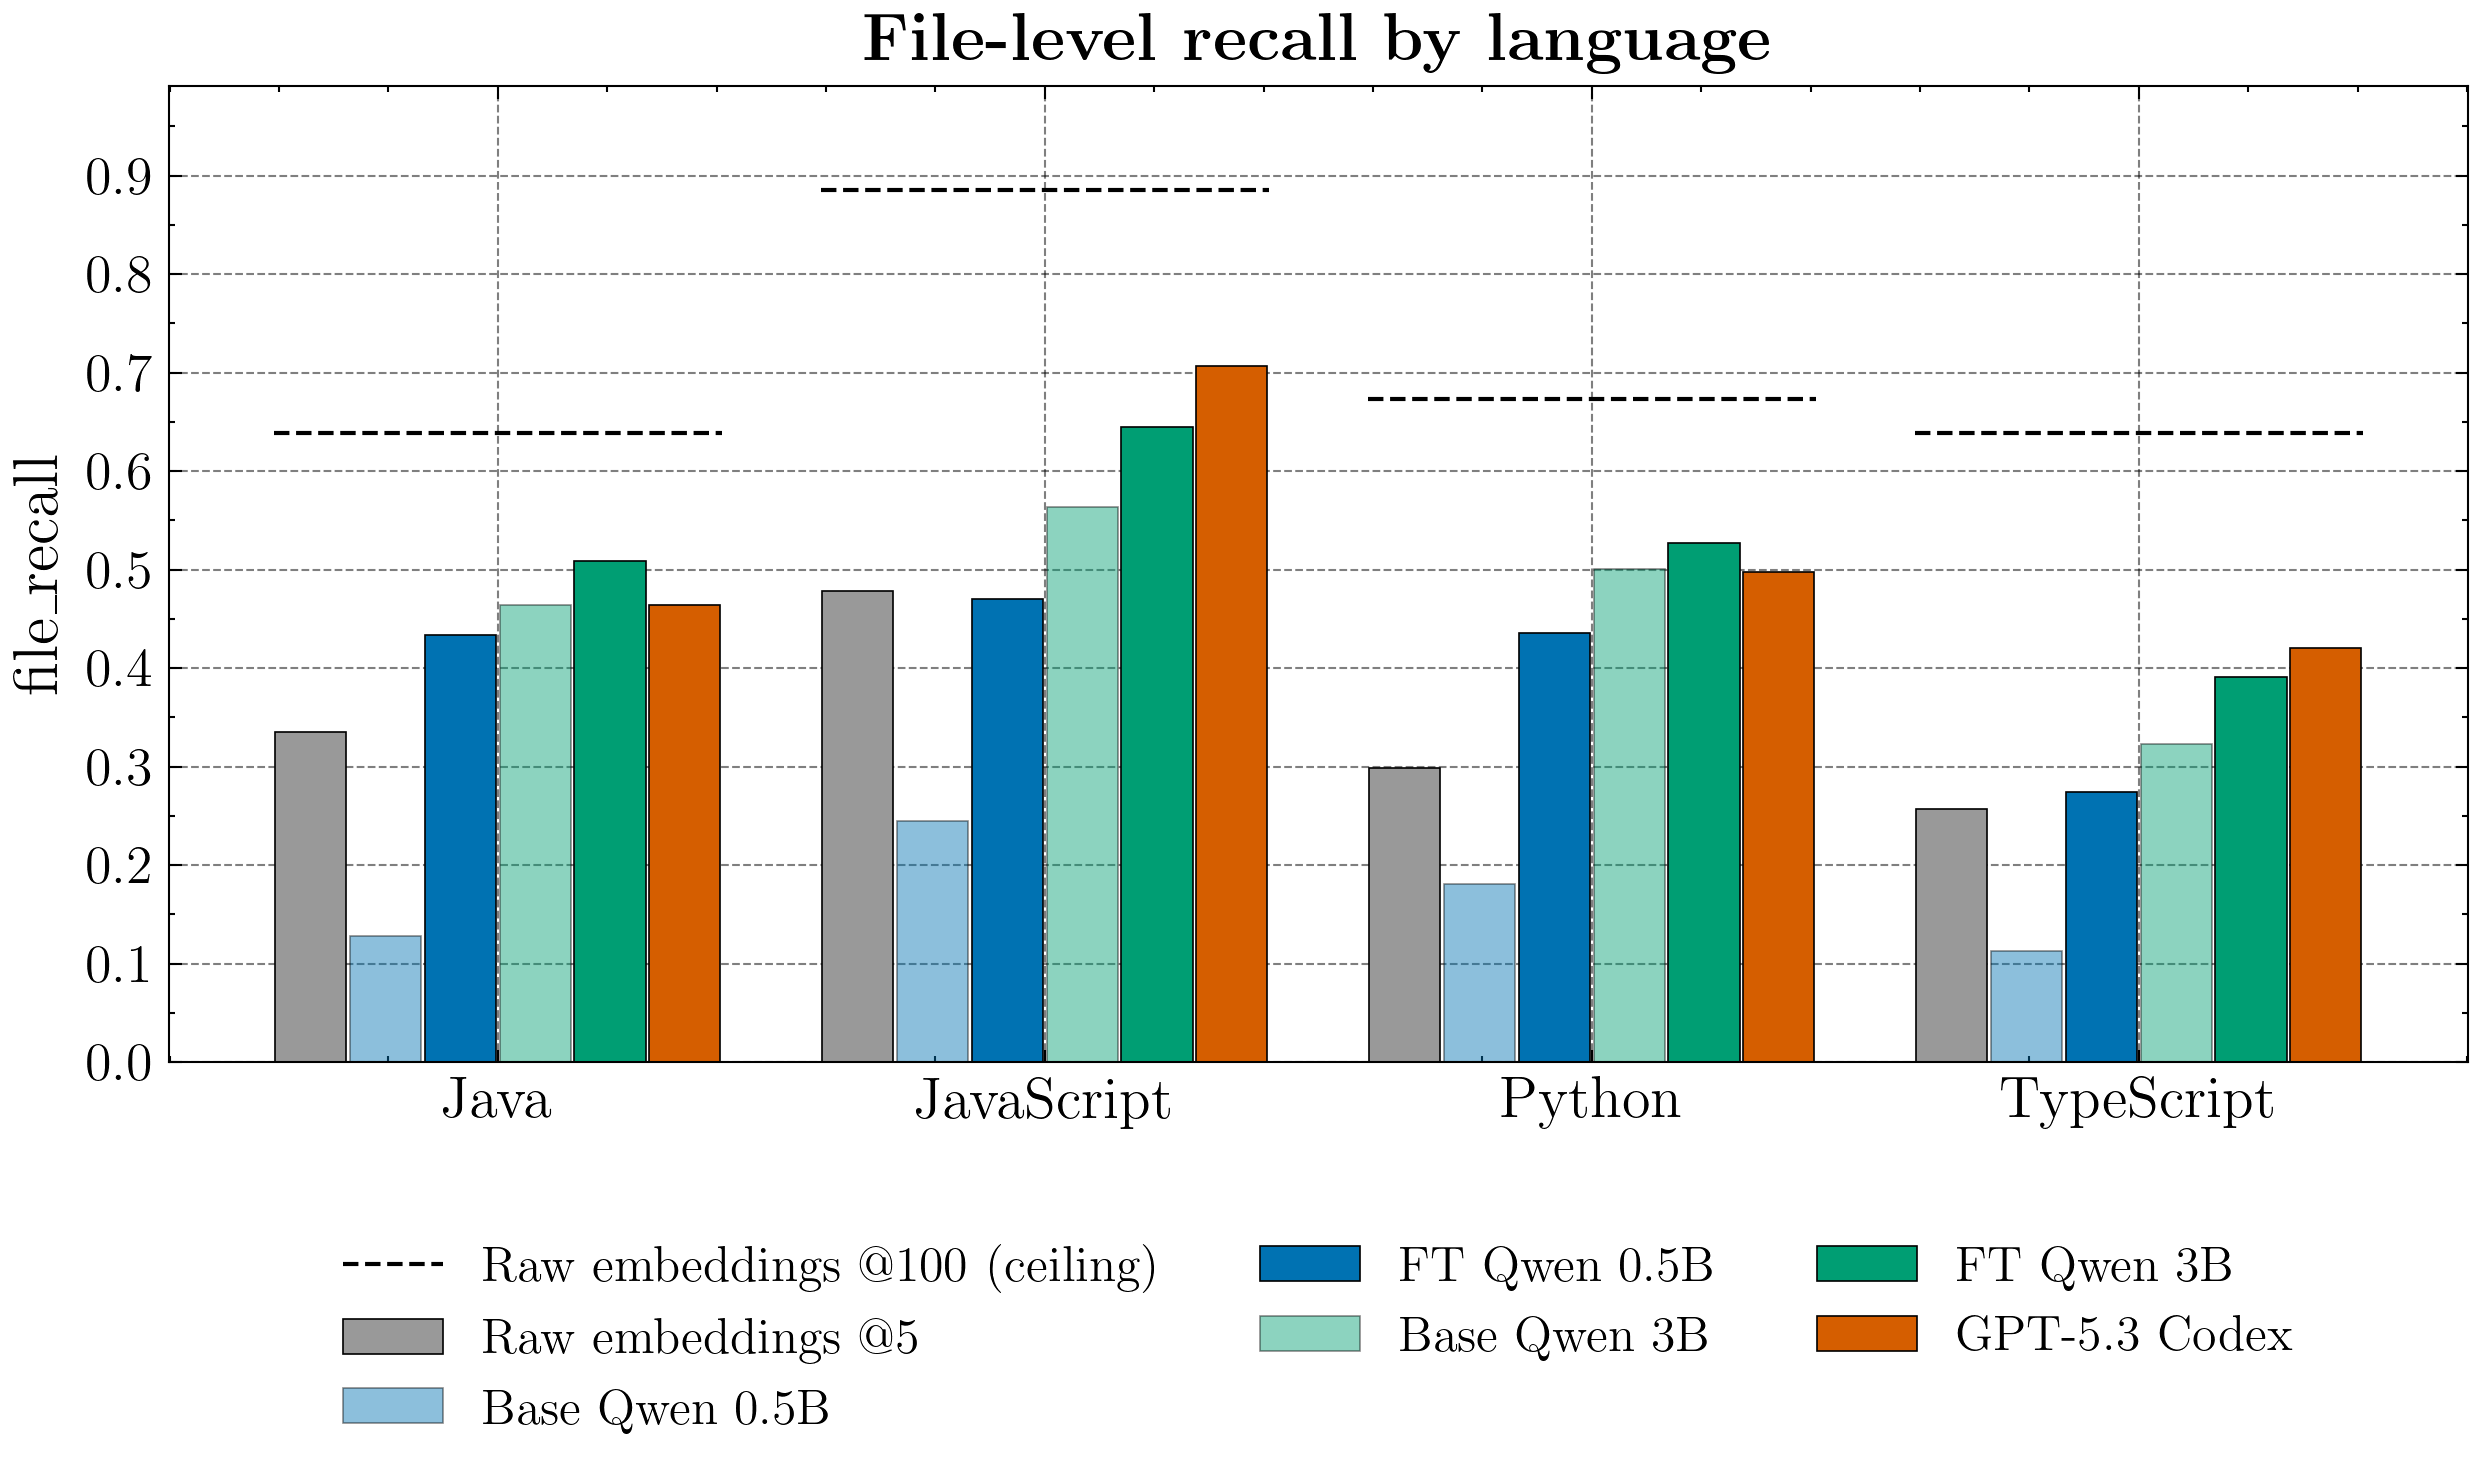
\includegraphics[width=0.85\textwidth]{imgs/reranker_file_recall.png}
\caption{Per-language file-level recall on SWE-PolyBench under
the windowed protocol of Figure~\ref{fig:scorer-func-recall}.
The dashed line marks the retrieval ceiling --- the recall
achievable if the gold function set lies in the top-$100$
retriever pool. The fine-tuned 3B scorer (FT Qwen 3B) matches
or exceeds GPT-5.3 Codex on Java and Python and tracks it within
a few points on JavaScript and TypeScript.}
\label{fig:scorer-file-recall}
\end{figure*}

\begin{figure*}[t]
\centering
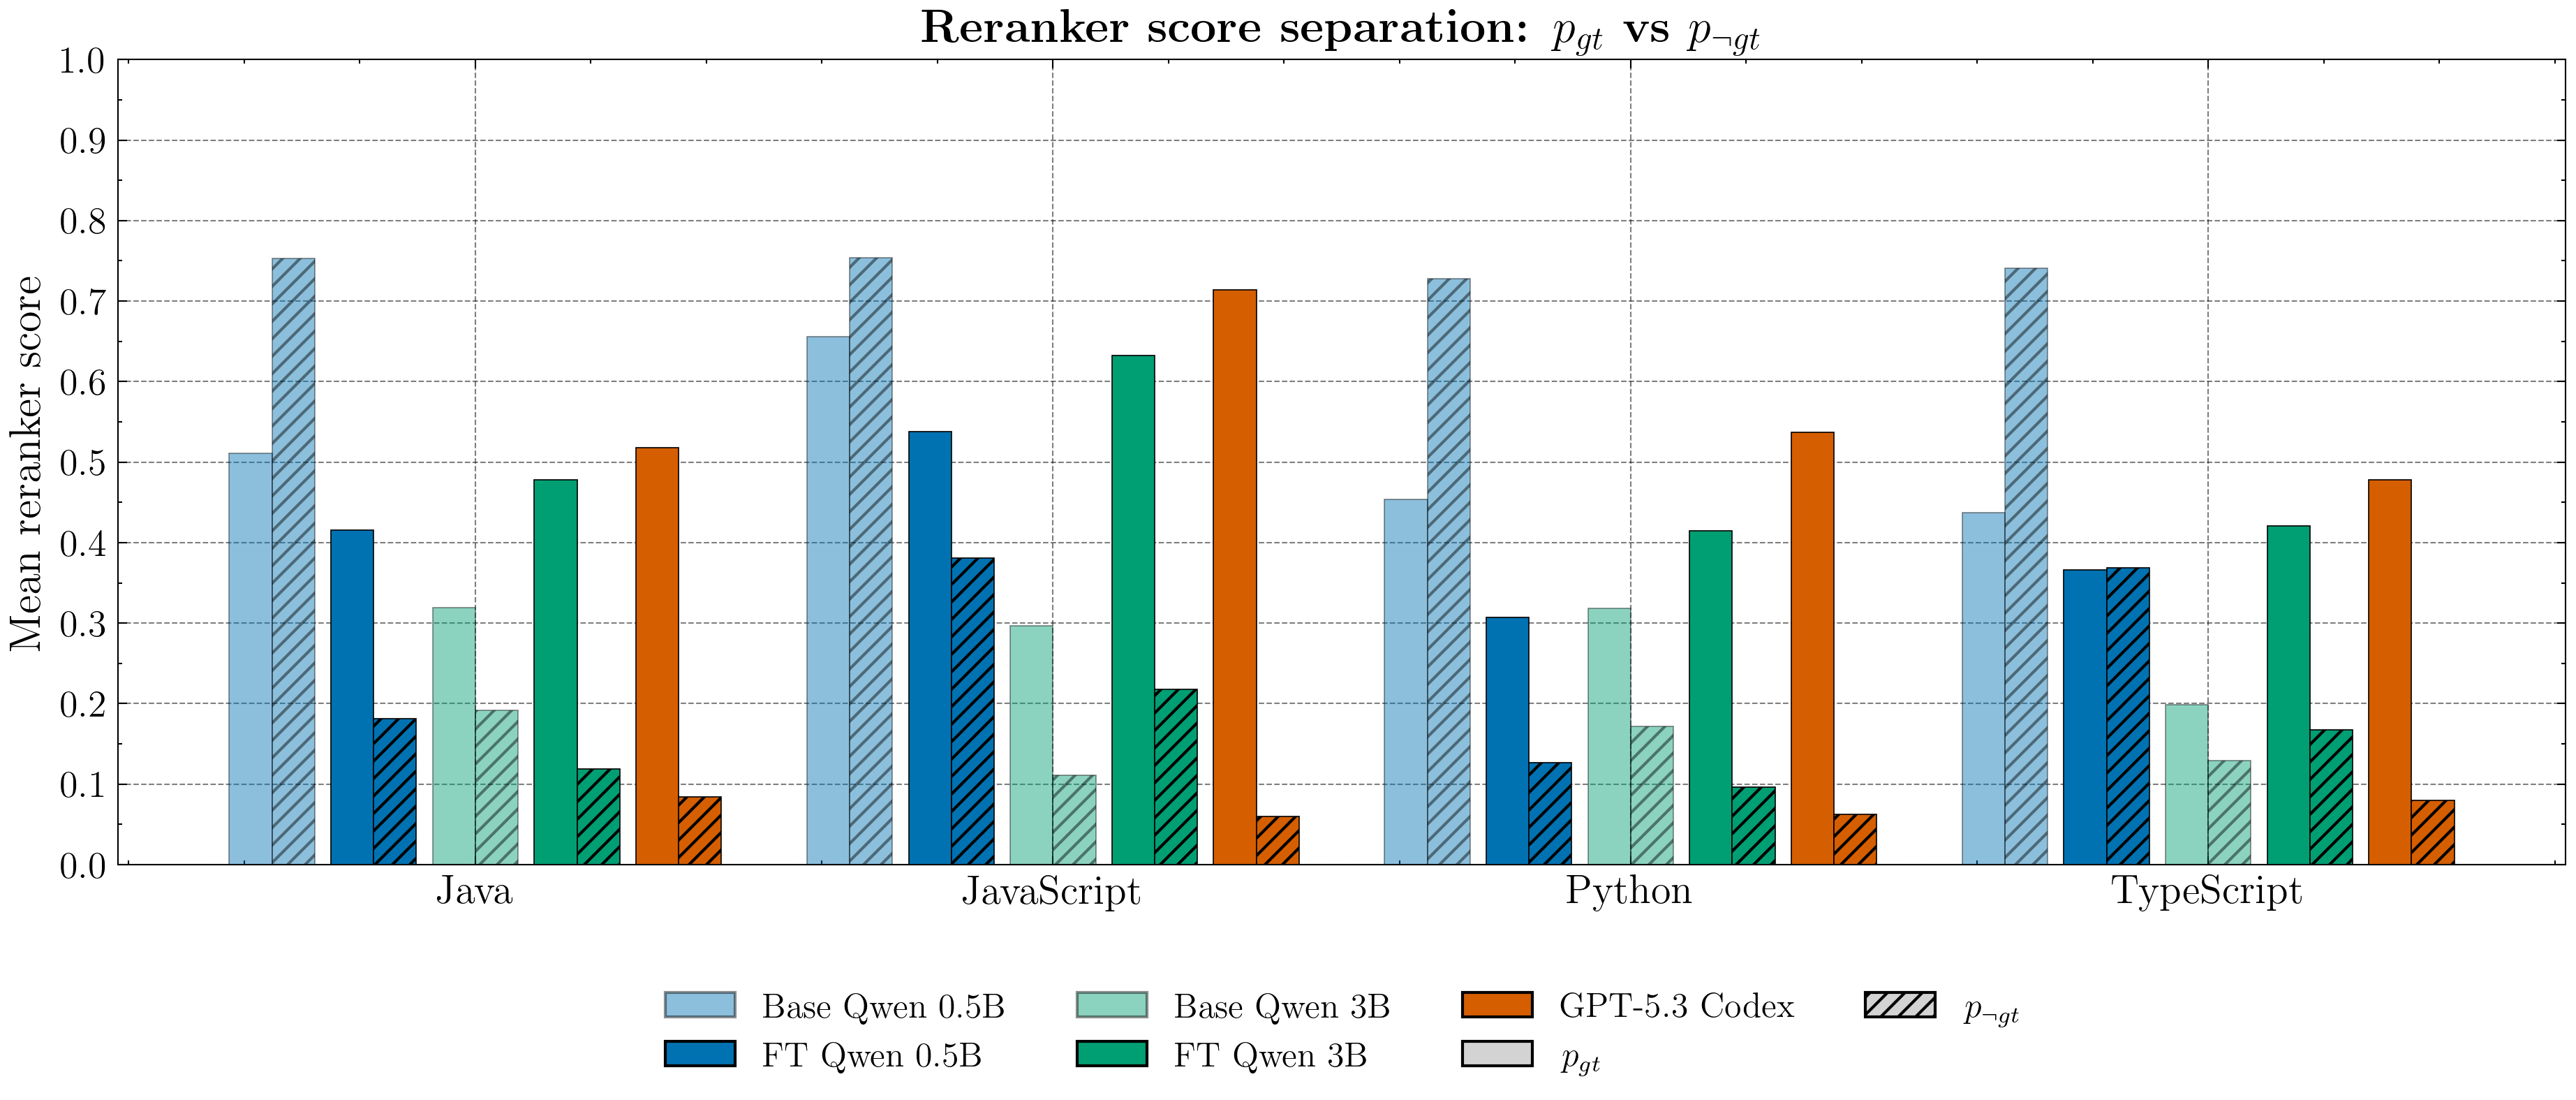
\includegraphics[width=0.85\textwidth]{imgs/reranker_score_separation.png}
\caption{Mean score on ground-truth candidates
($p_{gt}$, filled bars) vs.\ non-relevant candidates
($p_{\neg gt}$, hatched bars), averaged per language under the
same windowed protocol. A wider gap indicates better
discrimination between gold and non-gold. Fine-tuning widens
the separation at every model size: the base 0.5B model is
actively mis-calibrated --- it assigns $p_{\neg gt} > p_{gt}$
in every language --- whereas the fine-tuned 3B variant
achieves a separation comparable to GPT-5.3 Codex, with
$p_{gt}$ above $p_{\neg gt}$ by a margin of $0.25$--$0.45$.}
\label{fig:scorer-score-separation}
\end{figure*}

\section{AI Disclosure}
\label{app:ai}
% - The ACL-required statement of AI-tool usage. Generate it
%   with the academic-paper `disclosure` mode once drafting is
%   complete.
